\section{NetLogo Projekte}
Die Dokumentation der zwei Projekte erfolgt in folgender Form:
Zuerst wird die zugrundeliegende Idee erl"autert, dann werden einige Hinweise
gegeben, wie das Beispiel 
im Unterricht vermittelt werden kann und die Teilkomponenten
einer Beispiell"osung erl"autert. Im Ausblick werden Anregungen erl"autert wie
sie z.B. eifrigen Sch"ulerInnen vorgestellt werden k"onnen oder Zus"atze die
in einem etwaigen Begabten-Unterricht als eigenst"andige Arbeit von den
Sch"ulerInnen gel"ost werden kann. 

Es wird dabei davon ausgegangen, dass die Lernenden schon Erfahrung mit 
NetLogo und ein gewisses Grundverst"andnis von Musik bzw. Akustik haben. 
% Die untenstehenden Beispiele wurden gleichzeit daf"ur genutzt, die Implementierung
% der Befehle zu testen. 
\subsection{Rotierende Trommler}
\label{Bsp:Trommler}
\subsubsection{Idee}
In diesem Beispiel sollen mehrere Trommler trommelnd im Kreis marschieren. Dazu
soll unabh"angig von der Musik, die sie spielen die Position ver"andert werden.
Diese Positions"anderung soll nat"urlich auch h"orbar sein. Es sollen also die
Trommler die sich am linken Rand des Feldes aufhalten auch st"arker auf der 
linken Seite der Lautsprecher zu h"oren sein sollen. 

\subsubsection{Didaktische Aufbereitung}
Das Projekt soll Schritt f"ur Schritt mit den Sch"ulern erarbeitet werden.
Von der Grundidee eines Trommlers "uber einen kreisenden Agenten bzw.
kreise drehende Turtle hinzu mehreren im Kreis marschierenden Trommlern.

\begin{description}
\item[Der Trommler]: Der Trommler soll einen 4/4 Takt schlagen. Also wirklich
nur simpel auf jeden Takt-Schlag einmal auf seine Trommel hauen. Zus"atzlich
soll er immer die Eins in jedem Takt betonen. Es kann "uberlegt werden, diesen
Schritt mit MidiCSD\cite{MidiCSD} in Excel/OpenOffice durchzuf"uhren. Die
Lernenden k"onnen sich die Tonh"ohe selbst aussuchen. Die L"ange des Taktes
bestimmt die Dauer der einzelnen Noten. Es muss nur ein Takt von den Lernenden
modelliert werden, da der Dirigent diesen dann endlos abspielen lassen kann.
Wird mit Excel gearbeitet, kann "uber die Phraselanguage der Takt 
mehrmals kopiert und hinten angef"ugt werden um ihn so "ofter abzuspielen.
Gut eignen sich drei Takte. Die Lernenden sollten wissen, dass bei einem 4/4
Takt alle Noten gleich lang sein sollen. In der Beispiell"osung sind alle
Schl"age 200ms lang. 
\item[Im Kreis gehende Turtle] In Midi beginnen die Kan"ale f"ur Trommler bei
Zehn. Deshalb sollen im Modell die Turtles auch erst bei Zehn beginnen. Also
bis 13 erstellen und die nicht ben"otigten wieder zerst"oren. Das nebeneinander
Aufstellen ist sehr einfach: Die Turtles sollen vom Ursprung aus nach Rechts
gehen und sich dann in ihre Richtung drehen. Dazu sollen sie zuerst ins
rechte - obere Eck schauen und sich dann um 45 Grad nach rechts drehen. Nach
M"oglichkeit sollen die Lernenden auf diesen Schritt selbst kommen oder eine
Alternativl"osung bringen. Um die Turtles am Kreis zu postieren m"ussen sie
dann nur um einen von ihrer Nummer abh"angigen Betrag vorw"arts gehen. Auch
das soll gemeinsam mit den Lernenden entwickelt werden. Jede Turtle besitzt
eine aufsteigende Nummer die in der Variable who gespeichert ist. Diese kann
dann auch gleich verwendet werden um, wenn die Turtles gegen-gleich rotieren
sollen, die Ausrichtung vorzunehmen (left-Befehl $-1^{who}$). Anhand des
Umfanges muss nun berechnet werden wie weit sich jede Turtle nach vorne 
bewegen muss. Den Lernenden sollte klar sein, dass eine Turtle, die weiter 
aussen steht, einen weiteren Weg zur"uck legen muss. Auch dass sich die
Turtle kontinuierlich drehen muss sollte f"ur die Lernenden kein Problem 
darstellen. 
Je nach Niveau der Lernenden kann an dieser Stelle dann noch ein Regler f"ur die 
Geschwindigkeit eingebaut werden. 
\item[Akustische-Effekte] Einige Lernende werden vermutlich gleich bemerken,
dass wenn nun die Trommler eingebaut werden, das ganze nicht sehr realistisch
klingt. Daf"ur besitzt NetLogo nun den UpdatePosition Befehl. Die Lernenden
sollen darauf hingewiesen werden, dass wenn keine Variable f"ur den Kanal
verwendet wird mit $(who + 1)$ zu arbeiten ist. Das eignet sich sehr gut
um die Problematik der Null und Eins basierenden Indizes zu erl"autern. 

\end{description}


\subsubsection{Benutzer-Oberfl"ache}

\begin{figure}[htb]
	\centering
		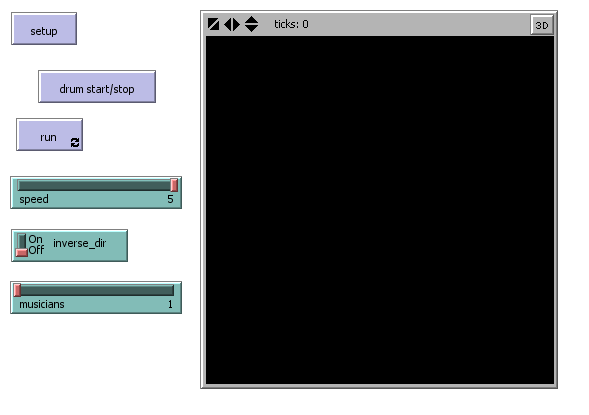
\includegraphics[scale=0.77]{fig/Trommler_interface.png}
	\caption{Trommler - Interface}
	\label{fig:Trommler.interface}
\end{figure}

Um das Programm zu starten ist es notwendig zuerst ''Setup'' und dann in 
beliebiger Reihenfolge ''drum start/stop'' und ''run'' zu dr"ucken. 
Der Knopf ''drum start/stop'' bewirkt dass der/die Trommler beginnen zu trommeln
, bzw. wieder aufh"oren zu trommeln. 

Ein Druck auf ''run'' l"asst die Trommler im Kreis marschieren, ein weiterer
Druck bewirkt, dass sie stehen bleiben. 

"Uber den Regler mit der Beschriftung speed kann die Geschwindigkeit der 
Trommler reguliert werden. Das kann auch passieren w"ahrend die Trommler schon
im Kreis marschieren.

Der Schalter ''inverse\_dir'' Entscheidet ob die Trommler alternierend gegengleich
marschieren oder nicht. Wir er auf ''On'' gesetzt, marschiert der erste Trommler
im Uhrzeigersinn, der Zweite gegen den Uhrzeigersinn und der Dritte wieder im
Uhrzeigersinn. Wird der Schalter umgelegt w"ahrend die Trommler schon marschieren
verlassen diese ihre Bahnen und beginnen von ihrem aktuellen Punkt aus wieder
in Kreisen zu marschieren, was an den Effekten der Akustik aber nichts "andert.

"Uber den Regler ''musicians'' wird die Anzahl der Trommler festgelegt. Nach 
einer "Anderung der Anzahl muss erneut auf ''setup'' gedr"uckt werden. 

\subsubsection{Funktionsweise}
Aufgrund der M"oglichkeiten, die die Erweiterung mit sich bringt ist der l"angste
Teil des Programm, die Setup-Prozedur. Sonst besteht das Programm noch aus zwei
weiteren Prozeduren: der Bewegung der Trommler und das Instruieren des Conductor.

Das Marschieren der Trommler ist simpel gehalten: Es wird lediglich berechnet,
wie weit jeder einzelne Trommler vorw"arts gehen muss, dann wird noch f"ur jeden
Trommler abh"angig davon ob sie alternierend gegengleich marschieren berechnet
wie weit er sich drehen muss. Dann wird jeder Trommler verschoben und ein
\lstinline|midi:updateposition| durchgef"uhrt. 

Das Instruieren des Conductor ist sehr einfach. Die \lstinline|drum|-Prozedur wird, von
einem Schalter am Interface aus aufgerufen. Wird noch nicht getrommelt, dh. die
Variable \lstinline|drumming| ist \lstinline|false|, wird 
"uber ein \lstinline|midi:conductor.start| der Conductor angewiesen mit dem
Musikst"uck zu beginnen und die Variable \lstinline|drumming| auf 
\lstinline|true| gesetzt. Im anderen Fall, also wenn schon getrommelt wird,
dh. die Variable \lstinline|drumming| ist \lstinline|true|, wird der Conductor
angewiesen das Musikst"uck zu beenden. Das passiert "uber den Befehl 
\lstinline|midi:conductor.stop|. Anschliesend wird noch \lstinline|drumming| auf
\lstinline|false| gesetzt. 

Das Setup des Models ist im Grunde auch einfach: F"ur drei Trommler werden die
Noten und die Instrumente definiert bzw. dem Conductor mitgeteilt (Befehle
\lstinline|midi:conductor.add.to.sheet| und \lstinline|midi:instrument|)


\subsubsection{Der Source Code im Detail}
Die Setup-Prozedur erstellt die Turtles die dann die Trommler darstellen und 
richtet das Midi-Interface sowie den Conductor ein. Es m"ussen die Instrumente
gesetzt werden, da Kanal elf und zw"olf nicht automatisch Percussion-Instrumente
verwenden. In diesem Beispiel habe ich die Variante gew"ahlt, dass der Conductor
angewiesen wird zu dirigieren, bzw. angewiesen wird mit dem Dirigieren 
aufzuh"oren. Das wird in der Prozedur \lstinline|drum| erledigt. Der Dirigent
arbeitet, nach dem er gestartet wurde im Hintergrund. (Achtung: Es sei an dieser
Stelle nochmal auf die Problematik mit Blocking-Calls hingewiesen. 
Siehe auch \ref{note-warning}). \lstinline|dosmg| f"ur Do-Something, l"asst
die Turtles wandern. 

\begin{lstlisting}[language=Logo]
extensions [midi]

globals [drumming doit]

to setup
  clear-all
  
  ;; sicher ist sicher
  midi:all.notes.off 10
  midi:all.notes.off 11
  midi:all.notes.off 12
  
  midi:conductor.clear.sheets
  midi:conductor.setplaymode.endless
  
  set drumming false
  set doit false
  
  midi:conductor.add.to.sheet 10 200 "midi:noteon 10 45 1"
  midi:conductor.add.to.sheet 10 200 "midi:noteon 10 45 0.7"
  midi:conductor.add.to.sheet 10 200 "midi:noteon 10 45 0.7"
  midi:conductor.add.to.sheet 10 200 "midi:noteon 10 45 0.7"
  ;midi:conductor.add.to.sheet 10 200 "midi:noteoff 10 45"
  
  if musicians > 1 [
  midi:conductor.add.to.sheet 11 200 "midi:noteon 11 46  1"
  midi:conductor.add.to.sheet 11 200 "midi:noteon 11 46  0.7"
  midi:conductor.add.to.sheet 11 200 "midi:noteon 11 46  0.7"
  midi:conductor.add.to.sheet 11 200 "midi:noteon 11 46  0.7"
  ]
  
  if musicians > 2 [
  midi:conductor.add.to.sheet 12 200 "midi:noteon 12 47 1"
  midi:conductor.add.to.sheet 12 200 "midi:noteon 12 47 0.7"
  midi:conductor.add.to.sheet 12 200 "midi:noteon 12 47 0.7"
  midi:conductor.add.to.sheet 12 200 "midi:noteon 12 47 0.7"
  ]
  
  ;setup the instruments
  midi:instrument 11 116
  midi:instrument 12 119
 
  ;create the turtles
  create-turtles (9 + musicians) [
    home
    facexy max-pxcor max-pycor
    rt 45
    fd who
    ifelse inverse_dir [lt (-1 ^ who) * 90 ][lt 90]
    set size 3
    ;; thicker line is easier to see
    set pen-size 3
    ;; leave a trail
    pen-down
  ]
  
  ; let the unused turtles die
  ask turtle 0 [die]
  ask turtle 1 [die]
  ask turtle 2 [die]
  ask turtle 3 [die]
  ask turtle 4 [die]
  ask turtle 5 [die]
  ask turtle 6 [die]
  ask turtle 7 [die]
  ask turtle 8 [die]
end

to dosmg
  ask turtles [
    let umf who * 2 * pi
    let turn 0.4 * speed
    
    fd 0.001 * speed * umf
    
    ifelse inverse_dir
     [lt (-1 ^ who) * turn]
     [lt turn]
    
    ; update turtle position
    midi:updateposition (who + 1)
  ]
  
  tick
end

to drum
  ifelse drumming = false[
    print "starting"
    midi:conductor.start
    set drumming true
  ]
  [
    print "stopping"
    midi:conductor.stop
    set drumming false
    set doit false
  ]
end
\end{lstlisting}





\subsubsection{Ausblick}
Ziel des Models ist es die Funktion ''midi:updateposition'' und den Conductor
auf seine ''start/stop''-F"ahigkeit zu testen. Aus diesem Grund ist das Model
sehr einfach gehalten. Ein paar Varianten um das Model zu erweitern sind:
\begin{itemize}
\item \emph{Orchester} Im aktuellen Model marschieren nur ein bis drei Trommler
im Kreis. Eine Erweiterung ist weitere Musiker mitspielen zu lassen. Das kann
"uber verschiedene Wege passieren: \begin{itemize}
\item \emph{komplett-statisch} Im Programm-Code wird festgelegt was ein
einzelner Musiker, wenn ausgew"ahlt, spielt. Das Interface wird um Switches f"ur
die einzelnen Musiker erweitert. 
\item \emph{teil-statisch} Das Interface wird erweitert, um die M"oglichkeit 
f"ur eine festgelegt Anzahl an Musikern, Noten und deren Werte einzugeben. Der
Programm-Code muss diese Werte dann in die Notenbl"atter schreiben und dem 
Conductor mitteilen. Achtung: Die Erweiterung des Interfaces um die Eingabe ist
bei weitem nicht einfach, da eine vern"unftige Struktur gefunden werden muss, 
wie die Noten und ihre Werte eingeben werden k"onnen. Auch im Programm-Code muss
dann einiges an Abfragen passieren ob einzelne Felder gesetzt sind
\item \emph{dynamisch} Die Musiker und ihre Noten werden "uber Dateien 
definiert. Das Programm wird so erweitert, dass es in einem Ordner nach Dateien
mit einem normierten Dateinamen sucht und aus diesen die Noten und ihre 
Noten-Werte ausliest. Als Format f"ur die Dateien ist ein einfaches CSV-Format
ausreichend. 
\end{itemize}
\item \emph{Marsch-Formationen} Anstatt die Trommler nur in Kreisbahnen gehen
zu lassen, kann das Model um die Funktionalit"at erweitert werden, dass sich
die Trommler auf selbst definierten Funktions-Bahnen bewegen. So kann das 
Interface um Eingabefelder erweitert werden wo f"ur jeden Trommler die Grenzen
f"ur die Funktion und die Funktion, welche abh"anig von einem Zeitparameter sein
sollte, eingegeben werden kann. Als programmiertechnische L"osung kann zB. in der
Setuproutine eine Liste mit Positions"anderungen angelegt werden, diese wird
durch schrittweise Berechnung, der einzelnen vom Benutzer eingegebenen 
Funktionen berechnet. 
\end{itemize}

\subsection{Rettungsauto}
\label{Bsp:Rettungsauto}
\subsubsection{Idee}
% Ein simuliertes Auto soll "uber den Bildschirm fahren und dabei das Martinshorn
% erklingen lassen. Es soll aber ein realistisches Modell sein, also der 
% Dopplereffekt simuliert werden.
Simulierte Rettungsautos sollen "uber den Bildschirm fahren und dabei das Martinshorn
erklingen lassen. Es soll aber ein nahezu realistisches
Model werden, was bedeutet, dass der Dopplereffekt ebenfalls simuliert
werden soll. Der Einfachheit halber gehen wir von einer kugelf"ormigen Welt aus,
die jedoch auf eine zweidimensionale Oberfl"ache abgebildet wird. Das bedeutet
nichts anderes, als das die normale NetLogo-Oberfl"ache verwendet werden kann,
die T"one sollen im zweidimensionalen Raum erscheinen und ein Auto, welches die
Welt auf der einen Seite verl"asst, soll auf der Anderen wieder hineinfahren. 
F"ur den Dopplereffekt soll davon ausgegangen werden, dass der Zuh"orer in
der Mitte, also auf der Koordinate $(0/0)$ steht. 

\subsubsection{Didaktische Aufbereitung}
Auch dieses Projekt sollte zuerst in eine Teilschritte zerlegt werden.
\begin{itemize}
\item Martins Horn
\item Dopplereffekt
\item Fahrendes Auto
\item Mehrere Autos
\end{itemize}
Wie im vorherigen Beispiel eignet sich auch hier der Schritt zuerst mit
MidiCSD die T"one zu entwickeln und dann erst mit NetLogo zu implementieren.

\begin{description}
\item[Martins Horn] Es soll ein "osterreichisches Rettungsauto modelliert werden.
Das Ziel-Instrument ist also eine Trompete. Die Lernenden sollen aber zuerst
selber raten und ausprobieren welches Instrument sich am Besten eignet. 
Ist das Instrument gefunden soll vom Ton mit dem Wert 60 aus der zweite Ton 
gefunden werden. Der Zugang kann entweder "uber das Experimentieren also das
Ausprobieren welcher Ton der Richtige ist, oder die Musik, also welches das 
richtige Intervall ist und wie dieses auf eine Midi-Tonh"ohe umgerechnet wird
gew"ahlt werden. 

\item[Dopplereffekt] Der Einfachheit halber sollte ein linearer Dopplereffekt
betrachtet werden. Sollten die Lernenden den Dopplereffekt nicht schon ausf"uhrlich
in Physik behandelt haben sollte eine Einf"uhrung in den Dopplereffekt und dessen
richtige Berechnung gegeben werden. "Uber Tabellen in Excel in denen mit der
Formel experimentiert wird, soll dann eine Formel f"ur die Berechnung entwickelt
werden. In der Beispiell"osung wird die skalierte Position des Autos mit $0.7$ 
multipliziert. Zu Beachten ist, dass in beiden F"allen mit $-1$ multipliziert wird,
da ein ansteigender Ton einen positiven Wert und ein abfallender Ton einen negativen
Wert erfordert. F"ur das verschieben des Tones gibt es den Befehl \lstinline|pitch.bend|
Dieser bekommt einen Wert zwischen $-1$ und $+1$. Pitchbending bedeutet nichts
anderes als das 'Beugen' der Tonh"ohe. 

\item[Fahrendes Auto] Das fahrende Auto ist in diesem Fall sehr einfach. Es muss
lediglich eine Turtle vorw"arts bewegt werden. Um das Model noch etwas realistischer
zu machen sollte zus"atzlich noch der UpdatePosition Befehl verwendet werden, damit
die Position auf der Ebene auch h"orbar gemacht wird. Das ganze kann "uber einen
Schieberegler der die Geschwindigkeit regeln soll und "uber den \lstinline|every|
-Befehl sehr sch"on und einfach gel"ost werden.

\item[Mehrere Autos] In diesem Schritt sollte am Besten ein Schieberegler f"ur
die Anzahl der Autos eingebaut werden. Im Setup "andert sich dann das statt
einer Turtle mehrere erstellt werden. Damit diese nicht alle parallel zu
einander fahren und auch nicht vom gleichen Punkt aus starten eignet sich
ein wiederholtes zur"uckgreifen auf Random. Im Code f"ur das Fahren "andert
sich nichts. F"ur das erstellen der Martinsh"orner ist jedoch ein kleiner
Trick erforderlich: Werden alle Autos mit den gleichen Werten f"ur die 
Notendauer versehen, klingt das nicht sehr gut. Anstatt jedes Auto bei 0 oder 1
beginnen zu lassen kann aber einfach mit \lstinline|who| begonnen werden. Das
bedeutet zwar, dass sich f"ur das zweite oder dritte Auto die T"one etwas
verschieben ist aber kaum h"orbar. Um das ganze echt Zeitversetzt zu machen,
w"aren aber einige Kunstgriffe notwendig. (Eine einfache L"osung ist aber
mit einem nicht h"orbaren Ton zu beginnen und dann in einer Schleife die T"one
f"ur das Martinshorn hinzuzuf"ugen und 'Playmode normal' auszuw"ahlen.)


\end{description}

\subsubsection{Benutzer-Oberfl"ache}

\begin{figure}[htb]
	\centering
		% width=304pt,height=225pt
		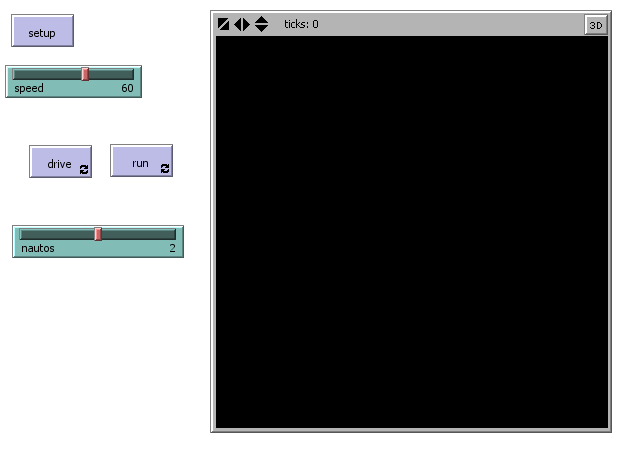
\includegraphics[scale=0.7]{fig/Rettungsauto_interface.jpg}
	\caption{Rettungsauto - Interface}
	\label{fig:Rettungsauto.interface}
\end{figure}

Die Abbildung \ref{fig:Rettungsauto.interface} zeigt die Oberfl"ache f"ur die 
Anwender des Modells. Links oben befindet sich der Knopf um das Modell zu 
initialisieren. Um die das Rettungsautofahren zulassen m"ussen die Kn"opfe
''run'' und ''drive'' gedr"uckt werden. Drive l"asst das Auto "uber die
Fl"ache fahren, w"ahrend ''run'' das Martinshorn aktiviert. 
Weiter unten befindet sich ein Regler um die Geschwindigkeit des Autos zu 
regeln. Sowie der Regler durch den sich die Anzahl der Autos festlegen l"asst. 
Diese "Anderung wird aber nur aktiv wenn erneut auf 'Setup' gedr"uckt wird. 

\subsubsection{Funktionsweise}
Das Grundprinzip des Models ist einfach: "Uber die zwei Kn"opfe werden 
unabh"angig von einander zwei Prozeduren wiederholt ausgef"uhrt. Die
Prozedur f"ur das Martinshorn enth"alt lediglich die Anweisung 
\lstinline|conductor.conduct| um das Abspielen der Midi-Befehle f"ur das 
Martinshorn zu bewirken. Die zweite Prozedur berechnet die Positions"anderung
anhand der Parameter Geschwindigkeit und vergangener Zeit. Anschlie"send 
schiebt sie die Schildkr"ote, welche das Rettungsauto repr"asentiert nach vorne
und f"uhrt ein Positions-Update f"ur die Schildkr"ote durch. 

\subsubsection{Der Source Code im Detail}
Die Setup-Prozedur erstellt das virtuelle Rettungsauto und richtet den Conductor
ein. Als Hilfsfunktion verwendet sie \lstinline|make.tatue| um die T"one f"ur
das Rettungsauto zu erzeugen. Das Beispiel verwendet in diesem Fall, als 
Unterschied zum Trommler-Beispiel die Variante den Conductor in jedem Schritt
einzeln aufzurufen und ihn dirigieren lassen. Damit kann das Auto unabh"angig von
seinem Martinshorn fahren lassen. Das Dirigieren wird in der kurzen Prozedur \lstinline|runit|
realisiert, das Fahren in \lstinline|drive|.

\begin{lstlisting}[language=Logo]
extensions [midi]

; globals [lasttick velocity lasttime]

turtles-own[channel]

to setup
  clear-all
  random-seed new-seed
  
  midi:conductor.clear.sheets
  midi:all.notes.off 1
  
  create-turtles nautos[
    set size 10
    setxy ((random 200) - 100) ((random 200) - 100)
    facexy ((random 100) - 50) ((random 50) - 25)
    set channel who + 1
    midi:updateposition channel
  ]
  
  make.tatue
    
  reset-timer
  ; set lasttime 0
end

to make.tatue
  ask turtles[
		midi:conductor.add.to.sheet channel 0 + who "midi:noteon 1 60 1"
		midi:conductor.add.to.sheet channel 250 "midi:noteoff 1 60"
		midi:conductor.add.to.sheet channel 10 "midi:noteon 1 65 1"
		midi:conductor.add.to.sheet channel 250 "midi:noteoff 1 65"
		
		midi:instrument channel 57
  ]
  
  midi:conductor.setplaymode.endless
end

to runit
  midi:conductor.conduct
end

to drive
  every 0.25 [
  ask turtles [
    fd speed * 0.1
    
    every 1 [ midi:updateposition channel]
    
    if xcor < 0 [
      midi:pitch.bend channel ( 0.7 / min-pxcor * xcor * -1 )
    ]
    if xcor = 0 [ midi:pitch.bend channel 0]
    if xcor > 0 [
      midi:pitch.bend channel ( 0.7 / max-pxcor * xcor * -1 )
    ]
  ]
  
  ]
  
  tick  
end
\end{lstlisting}


\subsubsection{Ausblick}
Das Modell zeigt zur Zeit nur elementare F"ahigkeiten der Midi-Extension, kann
aber nat"urlich beliebig erweitert werden. 
\begin{itemize}
\item \emph{Mehr Fahrzeuge: }
Das Modell kann nat"urlich um weitere Autos erweitert werden. So ist es 
m"oglich "uber den Dirigenten Notenbl"atter f"ur die verschiedenen Fahrzeuge
anzulegen. So kann das Model sehr einfach um Feuerwehr, Polizei, oder anderes
erweitert werden. Soll sich auch die Art der Fortbewegung "andern muss die 
drive-Prozedur ver"andert werden. 
\item \emph{Hindernisse: }
Im aktuellen Model fahren die Autos ungehindert durch die Welt. Durch einfache
"Anderungen am Modell k"onnten breeds als Hindernisse deklariert werden. F"ahrt
ein Auto auf eines von diesen auf, soll eine Aktion ausgef"uhrt werden (zB das
Auto soll wenden, also eine 180 Grad Drehung machen)
\item \emph{Fahrtverl"aufe: } 
In der aktuellen Implementierung kann lediglich der Startpunkt des Autos gesetzt
werden, nicht jedoch der Verlauf der Fahrt. Ein m"ogliche Erweiterung ist, dass
der Benutzer aus mehreren Funktionen ausw"ahlen oder diese auch selber eingeben 
kann, welche den Verlauf der Fahrt berechnen.
\item \emph{Genauerer Dopplereffekt: }
Der Dopplereffekt wird im vorliegenden Modell nur approximiert. Durch Literatur-Recherche und 
geringf"ugige "Anderungen am Code, kann sehr einfach eine bessere Ann"aherung
erreicht werden. 
\end{itemize}

